\documentclass[a4paper,uplatex,dvipdfmx,ja=standard,11pt]{bxjsarticle}
\setpagelayout{ignorehead}

\usepackage[dynamics]{PrettyLatexReport} % for dynamics seminar
%\usepackage{PrettyLatexReport} % for research seminar

\title{2016/12/02 ゼミ}
\author{Wernher Magnus Maximilian Freiherr von Braun}
\date{\today}
% 輪講(力学ゼミ)担当範囲
\contents{100}{110} % required only for dynamics seminar

% 章番号,式番号などの変更
%\setcounter{section}{3}
%\setcounter{subsection}{13}
%\setcounter{subsubsection}{4}	
%\setcounter{equation}{141}  

\begin{document}
	\maketitle
	
	\section{序論}
	We choose to go to the moon. We choose to go to the moon in this decade and do the other things, not because they are easy, but because they are hard, because that goal will serve to organize and measure the best of our energies and skills, because that challenge is one that we are willing to accept, one we are unwilling to postpone, and one which we intend to win, and the others, too.
	
	
	いろはにほへとちりぬるを
	わかよたれそつねならむ
	うゐのおくやまけふこえて
	あさきゆめみしゑひもせす
	
	色は匂へど 散りぬるを
	我が世誰ぞ 常ならむ
	有為の奥山 けふ越えて
	浅き夢見じ 酔ひもせず
	
	\paragraph{小見出し}\leavevmode\\
	\indent
	小見出しを入れたい場合の処理
	
	
	\section{引用}
	引用のテスト\cite{Stevenson2012,Tsukahara2016},\cite{konoue2005,schaubtext,yatsu2014pre,Isabelle}
\begin{figure}[h]
	\begin{subfigure}{0.5\linewidth}
		\centering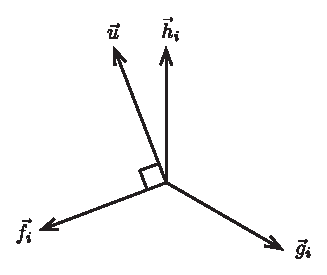
\includegraphics[width=5cm]{fig/fig1.eps}
		\caption{$\vec{f},\vec{g},\vec{h},\vec{u}$の関係}\label{fig:fig1}    % キャプションが図の下部に入る
	\end{subfigure}
	\begin{subfigure}{0.5\linewidth}
		\centering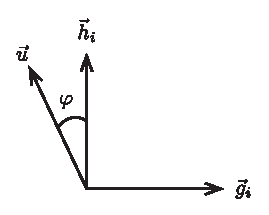
\includegraphics[width=5cm]{fig/fig2.eps}
		\caption{$\vec{g},\vec{h},\vec{u}$の関係}\label{fig:fig2}    % キャプションが図の下部に入る
	\end{subfigure}
	\caption{各ベクトルの幾何的関係}\label{fig:case4} 
\end{figure}

\bibliography{references}

\end{document} 